\documentclass[11pt,a4paper]{article}
\usepackage[T1]{fontenc}
\usepackage{geometry}
\usepackage{amsmath}
\usepackage{amssymb}
\usepackage{booktabs}
\usepackage{graphicx}
\usepackage[table]{xcolor}
\usepackage{array}
\usepackage{mathptmx}
\usepackage{listings}
\usepackage{hyperref}
\usepackage{tikz}
\usetikzlibrary{arrows.meta, positioning, fit, shapes.geometric, decorations.pathreplacing}

\geometry{margin=1in}

\tikzset{
  matbox/.style={draw, thick, minimum width=1.15cm, minimum height=1.15cm, align=center, font=\scriptsize, fill=gray!8},
  outbox/.style={draw, thick, minimum width=1.15cm, minimum height=1.15cm, align=center, font=\scriptsize, fill=green!12},
  kernbox/.style={draw, thick, rounded corners=2pt, minimum width=2.5cm, minimum height=1.2cm, align=center, font=\scriptsize,
                  fill=blue!7, text width=2.3cm},
  redbox/.style={draw, thick, rounded corners=2pt, align=center, font=\scriptsize, fill=red!12, minimum height=1.0cm},
  flowarrow/.style={-{Stealth[length=2.2mm, width=1.6mm]}, thick},
}

\definecolor{codebg}{gray}{0.95}
\lstset{basicstyle=\ttfamily\scriptsize, backgroundcolor=\color{codebg}, breaklines=true, frame=single, columns=fullflexible,
        showstringspaces=false, breakatwhitespace=false}

\title{Cholesky Factorization in Mixed Precision under NixNan\\
\large Where Lowering the Precision Loses Positive Definiteness, and What NixNan Reports}
\author{SC26 Tutorial / NixNan Experiments}
\date{}

\begin{document}
\maketitle

% ================================================================== 1
\section{Executive Summary}

This report documents the experiments E0--E7 of a mixed-precision Cholesky study for the SC26 tutorial. The tutorial
point is: \emph{if the precision of a Cholesky factorization is reduced without regard to the condition number, rounding can destroy the
small positive Schur-complement pivot that the algorithm needs; the factorization then reaches
$L_{jj}=\sqrt{S_{jj}}$ with $S_{jj}\le 0$ and produces Inf and NaN, which NixNan can locate.} All experiments ran on one NVIDIA GeForce RTX 3090
(compute capability 8.6, driver 595.99.02, CUDA 12.4), with NixNan (\url{https://github.com/parfloat/nixnan}) built from
the copy in \texttt{external/nixnan} (commit \texttt{ce35185}, 2026-09-26).

\begin{enumerate}
  \item \textbf{The failure is reproducible, fast and located by NixNan.} On $A_\delta=\mathbf{1}\mathbf{1}^T+\delta I$ ($n=256$, $\delta=2^{-12}$,
  $\kappa_2=1.05\times10^{6}$), storing the matrix in FP16, BF16 or TF32 rounds $1+\delta$ to $1$, so the stored matrix is the rank-one
  $\mathbf{1}\mathbf{1}^T$ and the \emph{second pivot is exactly zero}. The division by it gives Inf, then NaN, which travel through every later kernel to the output.
  A NixNan run takes about 3~s. FP32 factors the same matrix cleanly.
  \item \textbf{Where each format breaks} (Section~\ref{sec:e2}): BF16 storage from $\delta=2^{-8}$, FP16 from $2^{-11}$, TF32 from $2^{-12}$
  (its ties round away from zero, so it survives one step longer than FP16), FP32 from $2^{-24}$, FP64 from $2^{-53}$. In FP32 and FP64 the forward error
  exceeds $0.1$ long before: from $2^{-14}$ or $2^{-23}$ in FP32, depending on the code path.
  \item \textbf{A bad condition number does not guarantee an exception.} With true FP16 arithmetic at $\delta=2^{-10}$ and BF16 arithmetic at $\delta=2^{-7}$
  the factorization error is small, no pivot is non-positive, \textbf{NixNan reports no exception}, and the solution is garbage (forward error $16$).
  NixNan finds exceptions, not ill-conditioning.
  \item \textbf{Reading a NixNan report needs care} (Section~\ref{sec:nixnan}): in the naive FP32 run the first report is a \emph{discarded} \texttt{rsqrt(0)}
  (the IEEE \texttt{sqrtf} sequence computes \texttt{MUFU.RSQ} first and range-tests afterwards), a div0/Inf report that never reaches a result, not a NaN and not the defect;
  with \texttt{MUFU.SQRT} it is absent. FP16/BF16 division and square root run in FP32, so one source operation shows up in two precision sections;
  conversion opcodes are not instrumented; and some kernels' reports carry no source line.
  \item \textbf{Tensor cores (E4).} A blocked Cholesky with an FP32 panel and a WMMA trailing update (FP16, BF16 or TF32 inputs, FP32 accumulate) breaks at the same $\delta$ as the naive storage
  (BF16 $2^{-8}$, FP16 and TF32 $2^{-11}$) but \emph{later in the factorization}: first bad pivot 33 (block step 1). NixNan instruments the \texttt{HMMA} instructions (NaN on the A and B input operands), but the
  first report is the genuine NaN at the square root of a negative Schur diagonal; the tensor cores only see NaN after the factorization has failed. Without refinement the mixed-precision factor is inaccurate (forward error 0.05--1) long before it breaks.
  \item \textbf{Random matrices (E5).} On $Q\,\mathrm{diag}(\sigma)Q^T$ ($n=256$, $\kappa=10^{2}$--$10^{7}$, 5 seeds) the order is the same as on $A_\delta$: FP32 never fails; mixed precision with FP16 or TF32 inputs is inaccurate from $\kappa=10^{3}$ and breaks down at $10^{6}$; BF16 is inaccurate already at $10^{2}$ and breaks down at $10^{5}$; naive FP16 arithmetic breaks down from $10^{4}$.
  Every breakdown was caught by the code's own pivot test. The inaccurate runs are the silent ones, and NixNan reports nothing for two of the three kinds of them (mixed BF16 at $10^{2}$, mixed TF32 at $10^{3}$) and only panel subnormals for mixed FP16.
  \item \textbf{The histogram view (E6).} With \texttt{HISTOGRAM=1} a healthy run has millions of operands in the binades $2^{-14}$--$2^{-8}$ of the Schur-update kernel; the failing run has none, only exponent~0 and exactly-zero values, and the zero bin names the instruction.
  The histogram is an operand census, not a Schur-complement monitor. \texttt{FUNCTION\_WHITELIST} cuts a run from 2.9 to 0.8~s but needs the full demangled name.
  \item \textbf{An explicit pivot guard (E7).} Testing the relative pivot before the square root stops the factorization with the pivot index, before any NaN exists: on the guarded runs NixNan reports no NaN. It also stops the inaccurate runs NixNan cannot see.
  The threshold $\tau=c\,u$ encodes the accuracy the user wants; $c=100$ separated the E5 runs perfectly, but a held-out check ($\kappa=150$--$700$) shows that this was a gap in the grid and that $c=300$ is needed for the 1000-$\epsilon$ criterion.
  \item \textbf{Cost.} Custom kernels (5 distinct kernels per run) cost 3~s under NixNan; the existing cuSOLVER/cuBLAS-based \texttt{mpir\_gpu}
  costs 88~s. All experiments stay inside the planned budget of 1~minute native, 2~minutes with NixNan.
\end{enumerate}

Scope: E0--E7 as planned. Open points are listed in Section~\ref{sec:next}.

% ================================================================== 2
\section{Background and the Question}

The study started from a discussion document (\texttt{cg-and-cholesky-nixnan.pdf}, a chat transcript, not a reference) that compares conjugate gradients with Cholesky
factorization, observes that the dominant cost of a blocked Cholesky is the trailing update $A_{RR}\leftarrow A_{RR}-L_{Rk}L_{Rk}^T$, a symmetric rank-$k$ update that is
essentially a GEMM and therefore maps to \textbf{tensor cores}, and proposes a NixNan tutorial: factor a badly conditioned SPD matrix in lowered precision and watch the exceptions.
The proposal's core idea is kept; each of its claims was checked rather than assumed.

\begin{table}[h]
\centering\small
\begin{tabular}{p{5.1cm}p{1.9cm}p{7.2cm}}
\toprule
Claim in the document & Status & Result in this study\\
\midrule
$A_\delta=\mathbf{1}\mathbf{1}^T+\delta I$ is SPD with $\kappa_2=(n+\delta)/\delta$ & confirmed & $\kappa_2=1.049\times10^6$ analytically and from the eigenvalues of the stored matrix\\
$1+\delta$ rounds to 1 in FP16/TF32 below $2^{-11}$, in BF16 below $2^{-8}$ & confirmed, with a refinement & FP16/BF16 break exactly at the tie ($2^{-11}$, $2^{-8}$); TF32 with ties away from zero breaks one step later ($2^{-12}$)\\
FP32 is safe because $1+\delta$ rounds only below $2^{-24}$ & partly right & breakdown does occur at $2^{-24}$, but accuracy is lost earlier and LAPACK disagrees with our kernels between $2^{-16}$ and $2^{-22}$\\
An unguarded factorization of the rounded matrix has a zero second pivot, then $0/0$ & confirmed & first bad pivot is index 1 in every breakdown\\
NixNan identifies the invalid operation, not merely the bad residual & confirmed, with caveats & Section~\ref{sec:nixnan}\\
Bad conditioning does not guarantee an exception & confirmed & finite-but-wrong runs with no NixNan report (Section~\ref{sec:e3})\\
\bottomrule
\end{tabular}
\end{table}

% ================================================================== 3
\section{Implementation}

\subsection{Algorithm and kernels}

Right-looking Cholesky without pivoting, $A=LL^T$, in custom CUDA (file \texttt{chol\_study.cu}). Two code paths:

\begin{itemize}
  \item \textbf{unblocked}: per column $k$, \texttt{pivot\_kernel} ($L_{kk}=\sqrt{S_{kk}}$), \texttt{scale\_kernel} ($L_{ik}=S_{ik}/L_{kk}$), \texttt{rank1\_kernel}
  ($S_{ij}\mathrel{-}=L_{ik}L_{jk}$), then \texttt{forward\_kernel} ($Ly=b$) and \texttt{backward\_kernel} ($L^Tx=y$);
  \item \textbf{blocked} ($NB=32$): \texttt{potrf\_tile\_kernel} (diagonal tile in shared memory), \texttt{trsm\_panel\_kernel}, \texttt{syrk\_kernel}
  (trailing update; the slot where tensor cores enter in E4), and the same two substitution kernels.
\end{itemize}

\begin{center}
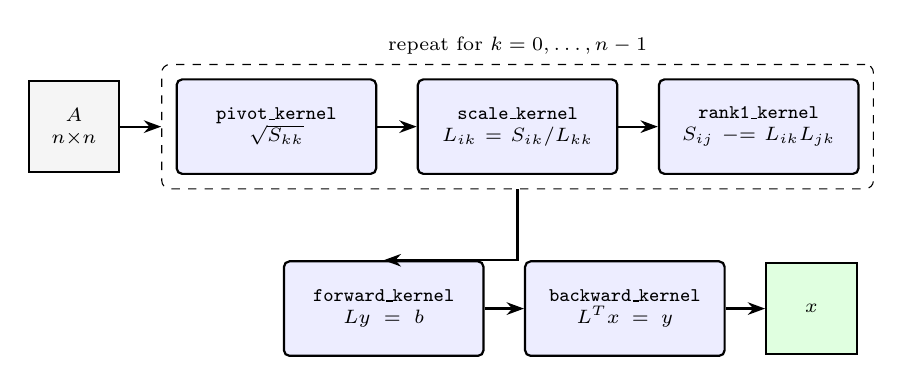
\begin{tikzpicture}[node distance=5mm]
  \node[matbox] (A) {$A$\\$n{\times}n$};
  \node[kernbox, right=7mm of A] (piv) {\texttt{pivot\_kernel}\\$\sqrt{S_{kk}}$};
  \node[kernbox, right=of piv] (sc) {\texttt{scale\_kernel}\\$L_{ik}=S_{ik}/L_{kk}$};
  \node[kernbox, right=of sc] (r1) {\texttt{rank1\_kernel}\\$S_{ij}\mathrel{-}=L_{ik}L_{jk}$};
  \node[draw, dashed, rounded corners=3pt, fit=(piv)(sc)(r1), inner sep=5pt, label={[font=\scriptsize]above:repeat for $k=0,\dots,n-1$}] (loop) {};
  \node[kernbox, below=9mm of loop, xshift=-1.7cm] (fw) {\texttt{forward\_kernel}\\$Ly=b$};
  \node[kernbox, right=of fw] (bw) {\texttt{backward\_kernel}\\$L^Tx=y$};
  \node[outbox, right=of bw] (x) {$x$};
  \draw[flowarrow] (A) -- (loop.west |- A.east); \draw[flowarrow] (piv) -- (sc); \draw[flowarrow] (sc) -- (r1);
  \draw[flowarrow] (loop.south) -- (loop.south |- fw.north) -- (fw.north);
  \draw[flowarrow] (fw) -- (bw); \draw[flowarrow] (bw) -- (x);
\end{tikzpicture}

\small Unblocked path. Five distinct kernels; the blocked path replaces the loop body by \texttt{potrf\_tile}, \texttt{trsm\_panel}, \texttt{syrk}.
\end{center}

\textbf{Tensor-core path} (file \texttt{chol\_tc.cu}, E4): the blocked path with $A$ and $L$ in FP32, \texttt{potrf\_tile} and \texttt{trsm\_panel} in FP32, and the trailing update
$A_{RR}\leftarrow A_{RR}-L_{Rk}L_{Rk}^T$ on tensor cores through WMMA, one warp per $16\times16$ tile, with FP32 accumulate. FP16 and BF16 inputs come from a rounded copy of the panel
(\texttt{convert\_panel\_kernel}; \texttt{wmma} $16{\times}16{\times}16$, \texttt{HMMA.16816.F32} and \texttt{.F32.BF16}); TF32 inputs are read from the FP32 panel and converted with \texttt{\_\_float\_to\_tf32}
(\texttt{wmma} $16{\times}16{\times}8$, \texttt{HMMA.1684.F32.TF32}). Substitutions are FP32.

The kernels do \textbf{not} guard the pivot. A non-positive pivot is only \emph{recorded} (\texttt{atomicMin} of its index, read back by the host);
the arithmetic goes on, so the bad pivot becomes Inf/NaN exactly as in unguarded code. In the arithmetic of the narrow formats (file \texttt{chol\_half.cu}, unblocked path only)
the update is one fused \texttt{\_\_hfma}, the scaling is \texttt{\_\_hdiv} and the pivot is \texttt{hsqrt}, for \texttt{\_\_half} or \texttt{\_\_nv\_bfloat16}.

\subsection{Matrices}

\begin{center}\small
\begin{tabular}{lllrr}
\toprule
name & definition & $\delta$ & $\kappa_2$, $n=256$ & $\kappa_2$, $n=64$\\
\midrule
M0 & $\mathbf{1}\mathbf{1}^T+\delta I$ & $2^{-6}$ & $1.6\times10^{4}$ & $4.1\times10^{3}$\\
M1 & $\mathbf{1}\mathbf{1}^T+\delta I$ & $2^{-12}$ & $1.0\times10^{6}$ & $2.6\times10^{5}$\\
\bottomrule
\end{tabular}
\end{center}

The eigenvalues are $n+\delta$ (once) and $\delta$ ($n-1$ times), so $A_\delta$ is SPD for every $\delta>0$. The matrices are written by
\texttt{gen\_chol\_matrices.py} (which can also produce random $Q\,\mathrm{diag}(\sigma)Q^T$ matrices for E5); the right-hand side is $b=A\mathbf{1}$, so the exact solution is $x=\mathbf{1}$.
The sweeps of E2 and E3 use the built-in $A_\delta$ with $\delta=2^{-e}$.

\subsection{Storage formats and metrics}

``Storage'' means every entry of $A$ is rounded to a narrow format and back before the factorization; the arithmetic is then FP32 (FP64 for the FP64 rows) unless
stated. FP16 and BF16 use round-to-nearest-even (\texttt{\_\_float2half\_rn}, \texttt{\_\_float2bfloat16\_rn}); TF32 keeps 10 mantissa bits with ties away from zero
(\texttt{cvt.rna.tf32.f32}, as \texttt{wmma::\_\_float\_to\_tf32}). Metrics are computed on the host in double:
$\|A-LL^T\|_F/\|A\|_F$ against the exact matrix, $\|b-Ax\|_2/\|b\|_2$ and $\|x-\mathbf{1}\|_2/\|\mathbf{1}\|_2$.
Status: \textbf{ok}; \textbf{inaccurate} (factorization error above $1000\,\varepsilon$ or forward error above $0.1$, a threshold chosen by me and arbitrary);
\textbf{breakdown} (the kernel saw a pivot $\le0$); \textbf{nan} (non-finite output the kernel did not notice).

% ================================================================== 4
\section{NixNan in Detail}\label{sec:nixnan}

\subsection{How it was run}

NixNan is a binary-instrumentation tool (NVBit) loaded with \texttt{LD\_PRELOAD}; it rewrites each kernel's SASS the first time the kernel launches and prints a report when the program exits.
No source change or recompilation is needed; the programs are built with \texttt{-lineinfo} so that source locations can be attributed.

\begin{center}\small
\begin{tabular}{p{4.6cm}p{9.2cm}}
\toprule
\texttt{LD\_PRELOAD=nixnan.so ./prog} & instrument every kernel; end-of-run report on stderr (all experiments)\\
\texttt{TIME\_KERNELS=1} & print every kernel's execution time; the first launch includes NVBit's instrumentation (E0)\\
\texttt{PRINT\_ILL\_INSTR=1} & print one line per exception with the SASS instruction that raised it (E3 traces)\\
\texttt{ENABLE\_FUN\_DETAIL=1} & put the kernel name on every line (E3 traces)\\
\texttt{LINE\_INFO} (default 1) & add \texttt{file:line} when the line table can be resolved\\
\texttt{NIXNAN\_TIMEOUT=N} & self-terminate after $N$ seconds (used for the 120~s reference run of \texttt{mpir\_gpu})\\
\bottomrule
\end{tabular}
\end{center}

\subsection{Anatomy of the end-of-run report}

The report has one section per precision (FP16, BF16, FP32, FP64) with five counters each (NaN, Infinity, $-$Infinity, Subnormal, Division by 0), and four memory sections that count
NaNs stored to global memory. Each counter reads ``\emph{unique} (\emph{repeats})'': the number of distinct instruction sites that raised it, and the number of further occurrences of
those sites. A clean run (matrix M1, FP32, unblocked, all counters zero):

\lstinputlisting[basicstyle=\ttfamily\tiny]{docs_gen/report_clean.txt}

The same matrix with FP16 storage (E3a, unblocked). Sections whose counters are all zero are dropped here (FP16, BF16, FP64 and the three other memory sections are zero): only the FP32 section and the FP32 memory section light up.

\lstinputlisting[basicstyle=\ttfamily\tiny]{docs_gen/report_f16_store.txt}

\noindent The same run with true FP16 arithmetic (E3b), again without the all-zero sections: \emph{two} precision sections are non-zero, and no memory section is.

\lstinputlisting[basicstyle=\ttfamily\tiny]{docs_gen/report_h16_arith.txt}

\subsection{The per-instruction trace}

With \texttt{PRINT\_ILL\_INSTR=1 ENABLE\_FUN\_DETAIL=1} every exception is printed with its operand number
(\texttt{0} = destination, \texttt{1\ldots n} = sources), the SASS instruction, the kernel and the type NixNan decoded the operand as. FP32 arithmetic on FP16-stored $A_\delta$ ($\delta=2^{-12}$), first lines:

\lstinputlisting[basicstyle=\ttfamily\tiny]{docs_gen/detail_f16_store.txt}

True FP16 arithmetic, same matrix, first lines:

\lstinputlisting[basicstyle=\ttfamily\tiny]{docs_gen/detail_h16_arith.txt}

The detail logs are summarised by the order in which kernels first appear and the number of lines each contributes (\emph{chain}):

\begin{center}\small
\begin{tabular}{lp{10.2cm}}
\toprule
run & chain (kernel: report lines), total lines, by kind\\
\midrule
FP16 storage, unblocked & \texttt{pivot\_kernel}: 6 $\to$ \texttt{scale\_kernel}: 29 $\to$ \texttt{rank1\_kernel}: 5 $\to$ \texttt{forward\_kernel}: 153 $\to$ \texttt{backward\_kernel}: 56; 249 lines (NaN 232, div0 4, Inf 13)\\
FP16 storage, blocked & \texttt{potrf\_tile\_kernel}: 159 $\to$ \texttt{trsm\_panel\_kernel}: 153 $\to$ \texttt{syrk\_kernel}: 68 $\to$ \texttt{forward\_kernel}: 153 $\to$ \texttt{backward\_kernel}: 56; 589 lines (NaN 567, div0 5, Inf 17)\\
FP16 arithmetic & \texttt{scale\_kernel}: 8 $\to$ \texttt{rank1\_kernel}: 4 $\to$ \texttt{pivot\_kernel}: 2 $\to$ \texttt{forward\_kernel}: 132 $\to$ \texttt{backward\_kernel}: 36; 182 lines (NaN 173, div0 3, Inf 6)\\
\bottomrule
\end{tabular}
\end{center}

\subsection{Cost of instrumentation}

NixNan instruments a kernel once, at its first launch, so the cost scales with the number of \emph{distinct} kernels, not with the number of launches. \texttt{TIME\_KERNELS=1} on M1, $n=256$, unblocked:

\lstinputlisting[basicstyle=\ttfamily\tiny]{docs_gen/time_kernels.txt}

Each first launch costs $\approx$0.3~s (it includes the NVBit rewrite); later launches are $\approx$20~$\mu$s. Five kernels therefore cost about 1.5~s of the 3~s run.
The library-based \texttt{mpir\_gpu/ir\_gpu} (cuSOLVER/cuBLAS), same size, ran in 0.5~s natively and 87.9~s under NixNan. Its NixNan run printed a complete report and then ended with
\texttt{terminate called without an active exception} and an abort; I did not investigate that.

\subsection{What the NixNan output does and does not mean}\label{sec:caveats}

\begin{enumerate}
  \item \textbf{The first report may be a discarded speculative operation.} IEEE \texttt{sqrtf} compiles to the sequence below (SASS of \texttt{pivot\_kernel}, trimmed). \texttt{MUFU.RSQ} runs for every
  input \emph{before} the argument is range-tested; the fast path (Newton refinement of the reciprocal square root) is taken only if the input is in range, otherwise a slow path returns the right special value
  ($\pm0\mapsto\pm0$, negative $\mapsto$ NaN). For $x=0$ the hardware really computes $\mathrm{rsqrt}(+0)=+\infty$, an IEEE division by zero, and NixNan reports it
  (\texttt{div0} on operand 1, the zero input; \texttt{infinity} on operand 0). The slow path then returns $0$: the infinity is \textbf{never used}, the program's result $\sqrt0=0$ is exact.
  It is a \emph{false positive of kind div0/Inf at the source level, not a NaN}: nothing at this site produces a NaN.

\lstinputlisting[basicstyle=\ttfamily\tiny]{docs_gen/sass_sqrt_ieee.txt}

  With \texttt{MUFU.SQRT} the sequence is a single instruction (plus denormal scaling) and nothing is reported at $\sqrt0$:

\lstinputlisting[basicstyle=\ttfamily\tiny]{docs_gen/sass_sqrt_fast.txt}

  I built the same sources with \texttt{-prec-sqrt=false} and re-ran E3a and E4 under NixNan (\texttt{./run\_chol\_story.sh sqrt}, \texttt{logs/sqrt/}):

\begin{center}\scriptsize\begin{tabular}{p{2.5cm}p{2.3cm}p{1.6cm}p{4.0cm}p{3.6cm}}
\toprule
case & sqrt compiled as & sqrt instruction & report at the sqrt site & first report in the run\\
\midrule
E3a: FP16 storage, pivot is $0$ & IEEE \texttt{sqrtf} & \texttt{MUFU.RSQ} & div0 (operand 1 = the $0$ input), infinity (operand 0 = $\mathrm{rsqrt}(0)$) & \texttt{MUFU.RSQ [div0]} in \texttt{pivot\_kernel}\\
E3a: FP16 storage, pivot is $0$ & \texttt{-prec-sqrt=false} & \texttt{MUFU.SQRT} & none at $\sqrt0$ (only NaN-input propagation later) & \texttt{MUFU.RCP [div0]} in \texttt{scale\_kernel}\\
E4: tensor-core update, pivot is $<0$ & IEEE \texttt{sqrtf} & \texttt{MUFU.RSQ} & NaN (operand 0 = the result) & \texttt{MUFU.RSQ [NaN]} in \texttt{potrf\_tile\_kernel}\\
E4: tensor-core update, pivot is $<0$ & \texttt{-prec-sqrt=false} & \texttt{MUFU.SQRT} & NaN (operand 0 = the result) & \texttt{MUFU.SQRT [NaN]} in \texttt{potrf\_tile\_kernel}\\
\bottomrule
\end{tabular}
\end{center}

  Consequences. In E3a with IEEE \texttt{sqrtf} the first report is this discarded \texttt{rsqrt(0)}; without it (\texttt{MUFU.SQRT}, and the FP16/BF16 \texttt{hsqrt} of E3b) the first report is \texttt{MUFU.RCP} in \texttt{scale\_kernel},
  the division by the zero pivot, which is \textbf{genuine} (its Inf or NaN reaches the output). For the square root of a \emph{negative} pivot (E4) the NaN at the sqrt is genuine in both builds. The remaining sqrt-site lines in the logs
  (NaN on operand 1 and 0 of the sqrt, \texttt{@P0 FADD.FTZ ... , 1}) are NaN \emph{inputs} propagated from earlier kernels, also genuine. Compare the \texttt{FFMA}-as-register-move artifact in the LU study:
  a SASS-level detector reports what the compiled code does, including speculative instructions.
  \item \textbf{One source operation, two precision sections.} FP16 and BF16 \texttt{\_\_hdiv} and \texttt{hsqrt} execute in FP32: the SASS of the FP16 build contains 39 \texttt{HFMA2}, 3 \texttt{MUFU.RCP},
  1 \texttt{MUFU.SQRT}, 6 \texttt{FFMA}, 3 \texttt{FMUL}, 7 \texttt{F2FP.PACK\_AB}, 3+4 \texttt{HSETP2}, 7 \texttt{HADD2}. The \texttt{HFMA2} updates are reported in the FP16 (or BF16) section, the division in the FP32 section.
  \item \textbf{Conversions are not instrumented.} The narrow-format rounding in E3a happens on the host, and NixNan does not instrument conversion opcodes (\texttt{F2F}, \texttt{F2FP}) in any case; the exception appears on the
  first arithmetic instruction that uses the converted value.
  \item \textbf{Memory sections:} the FP32-arithmetic runs report one memory NaN site (94\,655 repeats, unblocked). The FP16-arithmetic run reports none, consistent with nixnan's known gap that 16-bit stores (\texttt{STG.E.U16}) are not instrumented; I did not check the store opcode in this program.
  \item \textbf{Source lines are partial.} \texttt{file:line} is printed for the substitution kernels but not for \texttt{pivot\_kernel}, \texttt{scale\_kernel}, \texttt{rank1\_kernel} (nor the tile kernels). The cubin contains a line table (\texttt{nvdisasm -g}); the cause on the NixNan side was not found. Attribution is therefore by kernel and SASS instruction.
  \item \textbf{HMMA instructions are instrumented.} Exceptions in \texttt{HMMA} are reported per operand: operands 1 and 2 are the A and B inputs, operand 0 the accumulator (Section~\ref{sec:e4}). The type NixNan decodes decides the section: f16 (bf16) inputs land in the FP16 (BF16) section, TF32 inputs are 32-bit registers typed f32 and land in the FP32 section.
  \item \textbf{Silence is not correctness.} Where no pivot is non-positive and no value overflows, NixNan reports nothing even if the answer is wrong (Section~\ref{sec:e3}).
\end{enumerate}

% ================================================================== 5
\section{Experiments}

All runs: $n=256$ unless stated; logs in \texttt{logs/e0}\ldots\texttt{logs/e3}; every table below is generated from those logs by \texttt{make\_chol\_docs.py}.

\subsection{E0: run-time budget}

Design constraint: at most 1~minute natively and 2~minutes under NixNan per run, so the tutorial can run live.

\begin{center}\small\begin{tabular}{lrrrl}
\toprule
run (FP32) & native (s) & nixnan (s) & kernels & within budget\\
\midrule
M0\_n64\_f32\_unblocked & 0.4 & 2.2 & 5 & yes\\
M0\_n64\_f32\_blocked & 0.3 & 2.2 & 5 & yes\\
M0\_n256\_f32\_unblocked & 0.3 & 2.9 & 5 & yes\\
M0\_n256\_f32\_blocked & 0.3 & 3.0 & 5 & yes\\
M1\_n64\_f32\_unblocked & 0.3 & 2.1 & 5 & yes\\
M1\_n64\_f32\_blocked & 0.3 & 2.2 & 5 & yes\\
M1\_n256\_f32\_unblocked & 0.3 & 2.8 & 5 & yes\\
M1\_n256\_f32\_blocked & 0.3 & 3.0 & 5 & yes\\
\bottomrule
\end{tabular}
\end{center}

Custom kernels are far inside the budget; the NixNan time is dominated by the one-time instrumentation of 5 kernels. $n=1024$ looks affordable for these kernels (not run).

\subsection{E1: reference}

\begin{center}\small\begin{tabular}{llrrrr}
\toprule
 & & \multicolumn{2}{c}{M0 ($\kappa_2=1.6\times10^{4}$)} & \multicolumn{2}{c}{M1 ($\kappa_2=1.0\times10^{6}$)}\\
arithmetic & path & $\|A-LL^T\|/\|A\|$ & $\|x-1\|/\|1\|$ & $\|A-LL^T\|/\|A\|$ & $\|x-1\|/\|1\|$\\
\midrule
F64 & unblocked & $1.0\!\times\!10^{-16}$ & $1.1\!\times\!10^{-14}$ & $1.1\!\times\!10^{-16}$ & $3.1\!\times\!10^{-13}$\\
F64 & blocked & $9.5\!\times\!10^{-17}$ & $4.0\!\times\!10^{-13}$ & $1.1\!\times\!10^{-16}$ & $3.3\!\times\!10^{-13}$\\
F32 & unblocked & $1.3\!\times\!10^{-9}$ & $8.8\!\times\!10^{-6}$ & $1.3\!\times\!10^{-9}$ & $7.5\!\times\!10^{-6}$\\
F32 & blocked & $1.0\!\times\!10^{-7}$ & $5.6\!\times\!10^{-4}$ & $5.2\!\times\!10^{-8}$ & $1.8\!\times\!10^{-2}$\\
\bottomrule
\end{tabular}
\end{center}

All eight runs have status ok, no bad pivot, and \textbf{no NixNan exception} in any precision section or in memory. The matrices are valid and the kernels are right.
The forward error depends on the code path in FP32 (M1: $7.5\times10^{-6}$ unblocked, $1.8\times10^{-2}$ blocked) although both factorizations are accurate; it is the more sensitive metric.

\subsection{E2: where does each format break?}\label{sec:e2}

Sweep of $\delta=2^{-e}$ on $A_\delta$ ($\kappa_2=(n+\delta)/\delta$); FP32 arithmetic on the rounded matrix; u = unblocked, b = blocked.
ok / inacc (error above $1000\,\varepsilon$ or forward error above 0.1) / BRK (pivot $\le0$).

\begin{center}\scriptsize\begin{tabular}{rr|cc|cc|cc|cc}
\toprule
$e$ & $\kappa_2$ & \multicolumn{2}{c|}{FP32 storage} & \multicolumn{2}{c|}{TF32 storage} & \multicolumn{2}{c|}{FP16 storage} & \multicolumn{2}{c}{BF16 storage}\\
 &  & u & b & u & b & u & b & u & b\\
\midrule
2 & $1.0\!\times\!10^{3}$ & \cellcolor{green!15}ok & \cellcolor{green!15}ok & \cellcolor{green!15}ok & \cellcolor{green!15}ok & \cellcolor{green!15}ok & \cellcolor{green!15}ok & \cellcolor{green!15}ok & \cellcolor{green!15}ok\\
3 & $2.0\!\times\!10^{3}$ & \cellcolor{green!15}ok & \cellcolor{green!15}ok & \cellcolor{green!15}ok & \cellcolor{green!15}ok & \cellcolor{green!15}ok & \cellcolor{green!15}ok & \cellcolor{green!15}ok & \cellcolor{green!15}ok\\
4 & $4.1\!\times\!10^{3}$ & \cellcolor{green!15}ok & \cellcolor{green!15}ok & \cellcolor{green!15}ok & \cellcolor{green!15}ok & \cellcolor{green!15}ok & \cellcolor{green!15}ok & \cellcolor{green!15}ok & \cellcolor{green!15}ok\\
5 & $8.2\!\times\!10^{3}$ & \cellcolor{green!15}ok & \cellcolor{green!15}ok & \cellcolor{green!15}ok & \cellcolor{green!15}ok & \cellcolor{green!15}ok & \cellcolor{green!15}ok & \cellcolor{green!15}ok & \cellcolor{green!15}ok\\
6 & $1.6\!\times\!10^{4}$ & \cellcolor{green!15}ok & \cellcolor{green!15}ok & \cellcolor{green!15}ok & \cellcolor{green!15}ok & \cellcolor{green!15}ok & \cellcolor{green!15}ok & \cellcolor{green!15}ok & \cellcolor{green!15}ok\\
7 & $3.3\!\times\!10^{4}$ & \cellcolor{green!15}ok & \cellcolor{green!15}ok & \cellcolor{green!15}ok & \cellcolor{green!15}ok & \cellcolor{green!15}ok & \cellcolor{green!15}ok & \cellcolor{green!15}ok & \cellcolor{green!15}ok\\
8 & $6.6\!\times\!10^{4}$ & \cellcolor{green!15}ok & \cellcolor{green!15}ok & \cellcolor{green!15}ok & \cellcolor{green!15}ok & \cellcolor{green!15}ok & \cellcolor{green!15}ok & \cellcolor{red!25}BRK & \cellcolor{red!25}BRK\\
9 & $1.3\!\times\!10^{5}$ & \cellcolor{green!15}ok & \cellcolor{green!15}ok & \cellcolor{green!15}ok & \cellcolor{green!15}ok & \cellcolor{green!15}ok & \cellcolor{green!15}ok & \cellcolor{red!25}BRK & \cellcolor{red!25}BRK\\
10 & $2.6\!\times\!10^{5}$ & \cellcolor{green!15}ok & \cellcolor{green!15}ok & \cellcolor{green!15}ok & \cellcolor{green!15}ok & \cellcolor{green!15}ok & \cellcolor{green!15}ok & \cellcolor{red!25}BRK & \cellcolor{red!25}BRK\\
11 & $5.2\!\times\!10^{5}$ & \cellcolor{green!15}ok & \cellcolor{green!15}ok & \cellcolor{green!15}ok & \cellcolor{green!15}ok & \cellcolor{red!25}BRK & \cellcolor{red!25}BRK & \cellcolor{red!25}BRK & \cellcolor{red!25}BRK\\
12 & $1.0\!\times\!10^{6}$ & \cellcolor{green!15}ok & \cellcolor{green!15}ok & \cellcolor{red!25}BRK & \cellcolor{red!25}BRK & \cellcolor{red!25}BRK & \cellcolor{red!25}BRK & \cellcolor{red!25}BRK & \cellcolor{red!25}BRK\\
13 & $2.1\!\times\!10^{6}$ & \cellcolor{green!15}ok & \cellcolor{green!15}ok & \cellcolor{red!25}BRK & \cellcolor{red!25}BRK & \cellcolor{red!25}BRK & \cellcolor{red!25}BRK & \cellcolor{red!25}BRK & \cellcolor{red!25}BRK\\
14 & $4.2\!\times\!10^{6}$ & \cellcolor{green!15}ok & \cellcolor{orange!30}inacc & \cellcolor{red!25}BRK & \cellcolor{red!25}BRK & \cellcolor{red!25}BRK & \cellcolor{red!25}BRK & \cellcolor{red!25}BRK & \cellcolor{red!25}BRK\\
15 & $8.4\!\times\!10^{6}$ & \cellcolor{green!15}ok & \cellcolor{orange!30}inacc & \cellcolor{red!25}BRK & \cellcolor{red!25}BRK & \cellcolor{red!25}BRK & \cellcolor{red!25}BRK & \cellcolor{red!25}BRK & \cellcolor{red!25}BRK\\
16 & $1.7\!\times\!10^{7}$ & \cellcolor{green!15}ok & \cellcolor{green!15}ok & \cellcolor{red!25}BRK & \cellcolor{red!25}BRK & \cellcolor{red!25}BRK & \cellcolor{red!25}BRK & \cellcolor{red!25}BRK & \cellcolor{red!25}BRK\\
17 & $3.4\!\times\!10^{7}$ & \cellcolor{green!15}ok & \cellcolor{orange!30}inacc & \cellcolor{red!25}BRK & \cellcolor{red!25}BRK & \cellcolor{red!25}BRK & \cellcolor{red!25}BRK & \cellcolor{red!25}BRK & \cellcolor{red!25}BRK\\
18 & $6.7\!\times\!10^{7}$ & \cellcolor{green!15}ok & \cellcolor{orange!30}inacc & \cellcolor{red!25}BRK & \cellcolor{red!25}BRK & \cellcolor{red!25}BRK & \cellcolor{red!25}BRK & \cellcolor{red!25}BRK & \cellcolor{red!25}BRK\\
19 & $1.3\!\times\!10^{8}$ & \cellcolor{green!15}ok & \cellcolor{orange!30}inacc & \cellcolor{red!25}BRK & \cellcolor{red!25}BRK & \cellcolor{red!25}BRK & \cellcolor{red!25}BRK & \cellcolor{red!25}BRK & \cellcolor{red!25}BRK\\
20 & $2.7\!\times\!10^{8}$ & \cellcolor{green!15}ok & \cellcolor{orange!30}inacc & \cellcolor{red!25}BRK & \cellcolor{red!25}BRK & \cellcolor{red!25}BRK & \cellcolor{red!25}BRK & \cellcolor{red!25}BRK & \cellcolor{red!25}BRK\\
21 & $5.4\!\times\!10^{8}$ & \cellcolor{green!15}ok & \cellcolor{orange!30}inacc & \cellcolor{red!25}BRK & \cellcolor{red!25}BRK & \cellcolor{red!25}BRK & \cellcolor{red!25}BRK & \cellcolor{red!25}BRK & \cellcolor{red!25}BRK\\
22 & $1.1\!\times\!10^{9}$ & \cellcolor{green!15}ok & \cellcolor{orange!30}inacc & \cellcolor{red!25}BRK & \cellcolor{red!25}BRK & \cellcolor{red!25}BRK & \cellcolor{red!25}BRK & \cellcolor{red!25}BRK & \cellcolor{red!25}BRK\\
23 & $2.1\!\times\!10^{9}$ & \cellcolor{orange!30}inacc & \cellcolor{orange!30}inacc & \cellcolor{red!25}BRK & \cellcolor{red!25}BRK & \cellcolor{red!25}BRK & \cellcolor{red!25}BRK & \cellcolor{red!25}BRK & \cellcolor{red!25}BRK\\
24 & $4.3\!\times\!10^{9}$ & \cellcolor{red!25}BRK & \cellcolor{red!25}BRK & \cellcolor{red!25}BRK & \cellcolor{red!25}BRK & \cellcolor{red!25}BRK & \cellcolor{red!25}BRK & \cellcolor{red!25}BRK & \cellcolor{red!25}BRK\\
25 & $8.6\!\times\!10^{9}$ & \cellcolor{red!25}BRK & \cellcolor{red!25}BRK & \cellcolor{red!25}BRK & \cellcolor{red!25}BRK & \cellcolor{red!25}BRK & \cellcolor{red!25}BRK & \cellcolor{red!25}BRK & \cellcolor{red!25}BRK\\
26 & $1.7\!\times\!10^{10}$ & \cellcolor{red!25}BRK & \cellcolor{red!25}BRK & \cellcolor{red!25}BRK & \cellcolor{red!25}BRK & \cellcolor{red!25}BRK & \cellcolor{red!25}BRK & \cellcolor{red!25}BRK & \cellcolor{red!25}BRK\\
\bottomrule
\end{tabular}
\end{center}

\begin{center}\small\begin{tabular}{lllrrl}
\toprule
arithmetic & storage & path & first not-ok $e$ & $\kappa_2$ & status (cause)\\
\midrule
FP32 & BF16 & blocked & 8 & $6.6\!\times\!10^{4}$ & breakdown (storage)\\
FP32 & BF16 & unblocked & 8 & $6.6\!\times\!10^{4}$ & breakdown (storage)\\
FP32 & FP16 & blocked & 11 & $5.2\!\times\!10^{5}$ & breakdown (storage)\\
FP32 & FP16 & unblocked & 11 & $5.2\!\times\!10^{5}$ & breakdown (storage)\\
FP32 & TF32 & blocked & 12 & $1.0\!\times\!10^{6}$ & breakdown (storage)\\
FP32 & TF32 & unblocked & 12 & $1.0\!\times\!10^{6}$ & breakdown (storage)\\
FP32 & FP32 & blocked & 14 & $4.2\!\times\!10^{6}$ & inaccurate (arithmetic), breakdown at 24\\
FP32 & FP32 & unblocked & 23 & $2.1\!\times\!10^{9}$ & inaccurate (arithmetic), breakdown at 24\\
FP64 & FP64 & blocked & 43 & $2.3\!\times\!10^{15}$ & inaccurate (arithmetic), breakdown at 53\\
FP64 & FP64 & unblocked & 52 & $1.2\!\times\!10^{18}$ & inaccurate (arithmetic), breakdown at 53\\
\bottomrule
\end{tabular}
\end{center}

\begin{itemize}
  \item \textbf{Storage breakdown} occurs where $1+\delta$ falls on a tie that rounds to 1: $2^{-8}$ (BF16), $2^{-11}$ (FP16). TF32 with ties away from zero rounds $1+2^{-11}$ up to $1+2^{-10}$ and fails one step later.
  The rounding mode of the tensor-core inputs therefore moves the threshold.
  \item \textbf{Demo point:} $\delta=2^{-12}$ (M1): FP32 ok on both paths while TF32, FP16 and BF16 all break. At $\delta=2^{-10}$ FP16 and TF32 are still ok, BF16 breaks.
  \item \textbf{The FP32 thresholds are implementation-dependent.} LAPACK \texttt{spotrf} (SciPy) reports ``not positive definite'' for $e=16$--22 where our kernels do not; for TF32, FP16 and BF16 the CPU and GPU agree at every $e$ (those fail at storage).
  $A_\delta$ keeps the form $s\,\mathbf{1}\mathbf{1}^T+\delta' I$ after every elimination step, which makes errors benign for some operation orders. Thresholds measured on it show how the failure looks, not where it will occur in general.
  \item The FP32 blocked path is not monotone (e=16 is ok between inaccurate neighbours). In FP64 the breakdown at $e=53$ is the matrix itself losing $\delta$ when built in double; its ``arithmetic'' label is loose.
\end{itemize}

NixNan on chosen points (FP32 arithmetic; the rows for FP16, BF16 and TF32 are identical because all three produce the same rounded matrix $\mathbf{1}\mathbf{1}^T$):

\begin{center}\scriptsize\begin{tabular}{llllp{7.3cm}}
\toprule
storage & $e$ & path & status & nixnan: non-zero counters, unique (repeats)\\
\midrule
BF16 & 12 & blocked & breakdown & FP32 NaN 566 (689\,040), FP32 Inf 17 (24), FP32 Div0 5 (11), FP32 Memory NaN 1 (2\,463)\\
BF16 & 12 & unblocked & breakdown & FP32 NaN 231 (675\,688), FP32 Inf 13 (28), FP32 Div0 4 (11), FP32 Memory NaN 1 (94\,655)\\
BF16 & 8 & blocked & breakdown & FP32 NaN 566 (689\,040), FP32 Inf 17 (24), FP32 Div0 5 (11), FP32 Memory NaN 1 (2\,463)\\
BF16 & 8 & unblocked & breakdown & FP32 NaN 231 (675\,688), FP32 Inf 13 (28), FP32 Div0 4 (11), FP32 Memory NaN 1 (94\,655)\\
FP16 & 11 & blocked & breakdown & FP32 NaN 566 (689\,040), FP32 Inf 17 (24), FP32 Div0 5 (11), FP32 Memory NaN 1 (2\,463)\\
FP16 & 11 & unblocked & breakdown & FP32 NaN 231 (675\,688), FP32 Inf 13 (28), FP32 Div0 4 (11), FP32 Memory NaN 1 (94\,655)\\
FP16 & 12 & blocked & breakdown & FP32 NaN 566 (689\,040), FP32 Inf 17 (24), FP32 Div0 5 (11), FP32 Memory NaN 1 (2\,463)\\
FP16 & 12 & unblocked & breakdown & FP32 NaN 231 (675\,688), FP32 Inf 13 (28), FP32 Div0 4 (11), FP32 Memory NaN 1 (94\,655)\\
FP32 & 12 & blocked & ok & no exceptions\\
FP32 & 12 & unblocked & ok & no exceptions\\
FP32 & 14 & blocked & inaccurate & no exceptions\\
FP32 & 23 & unblocked & inaccurate & no exceptions\\
TF32 & 12 & blocked & breakdown & FP32 NaN 566 (689\,040), FP32 Inf 17 (24), FP32 Div0 5 (11), FP32 Memory NaN 1 (2\,463)\\
TF32 & 12 & unblocked & breakdown & FP32 NaN 231 (675\,688), FP32 Inf 13 (28), FP32 Div0 4 (11), FP32 Memory NaN 1 (94\,655)\\
\bottomrule
\end{tabular}
\end{center}

\subsection{E3: naive reduced precision}\label{sec:e3}

\paragraph{E3a: FP16/BF16 storage, FP32 arithmetic, $\delta=2^{-12}$.}

\begin{center}\scriptsize\begin{tabular}{lllp{4.6cm}p{3.6cm}}
\toprule
storage & path & status & nixnan report & first exception\\
\midrule
BF16 & blocked & breakdown, bad pivot 1 & FP32 NaN 566 (689\,040), FP32 Inf 17 (24), FP32 Div0 5 (11), FP32 Memory NaN 1 (2\,463) & \texttt{MUFU.RSQ R3, R0}, div0, potrf\_tile\_kernel\\
BF16 & unblocked & breakdown, bad pivot 1 & FP32 NaN 231 (675\,688), FP32 Inf 13 (28), FP32 Div0 4 (11), FP32 Memory NaN 1 (94\,655) & \texttt{MUFU.RSQ R7, R0}, div0, pivot\_kernel\\
FP16 & blocked & breakdown, bad pivot 1 & FP32 NaN 566 (689\,040), FP32 Inf 17 (24), FP32 Div0 5 (11), FP32 Memory NaN 1 (2\,463) & \texttt{MUFU.RSQ R3, R0}, div0, potrf\_tile\_kernel\\
FP16 & unblocked & breakdown, bad pivot 1 & FP32 NaN 231 (675\,688), FP32 Inf 13 (28), FP32 Div0 4 (11), FP32 Memory NaN 1 (94\,655) & \texttt{MUFU.RSQ R7, R0}, div0, pivot\_kernel\\
\bottomrule
\end{tabular}
\end{center}

The stored matrix is $\mathbf{1}\mathbf{1}^T$; $L_{i1}=1$ for all $i$; the update gives $S=0$; $\sqrt{0}=0$; then $0/0$. The NaNs travel through the update (\texttt{rank1} or \texttt{trsm}/\texttt{syrk}) and both substitutions.
FP16 and BF16 storage produce identical counts. The first line of each trace is the $\sqrt0$ expansion (Section~\ref{sec:caveats}); the first real failure is the next kernel's division by the zero pivot.

\paragraph{E3b: true FP16/BF16 arithmetic (unblocked).}

\begin{center}\small
FP16 arithmetic\\[1mm]\begin{tabular}{lccccccccccccc}
\toprule
$e$ & 2 & 3 & 4 & 5 & 6 & 7 & 8 & 9 & 10 & 11 & 12 & 13 & 14\\
\midrule
status & \cellcolor{green!15}ok & \cellcolor{green!15}ok & \cellcolor{green!15}ok & \cellcolor{green!15}ok & \cellcolor{green!15}ok & \cellcolor{green!15}ok & \cellcolor{green!15}ok & \cellcolor{green!15}ok & \cellcolor{orange!30}inacc & \cellcolor{red!25}BRK & \cellcolor{red!25}BRK & \cellcolor{red!25}BRK & \cellcolor{red!25}BRK\\
\bottomrule
\end{tabular}
\\[3mm]
BF16 arithmetic\\[1mm]\begin{tabular}{lccccccccccccc}
\toprule
$e$ & 2 & 3 & 4 & 5 & 6 & 7 & 8 & 9 & 10 & 11 & 12 & 13 & 14\\
\midrule
status & \cellcolor{orange!30}inacc & \cellcolor{orange!30}inacc & \cellcolor{orange!30}inacc & \cellcolor{orange!30}inacc & \cellcolor{orange!30}inacc & \cellcolor{orange!30}inacc & \cellcolor{red!25}BRK & \cellcolor{red!25}BRK & \cellcolor{red!25}BRK & \cellcolor{red!25}BRK & \cellcolor{red!25}BRK & \cellcolor{red!25}BRK & \cellcolor{red!25}BRK\\
\bottomrule
\end{tabular}

\end{center}

\begin{center}\scriptsize\begin{tabular}{llllp{5.4cm}}
\toprule
arithmetic & $\delta$ & status & forward error & nixnan report\\
\midrule
FP16 & $2^{-10}$ & inaccurate & $1.6\!\times\!10^{1}$ & no exceptions\\
FP16 & $2^{-12}$ & breakdown (bad pivot 1) & NaN & FP16 NaN 156 (636\,986), FP32 NaN 17 (8\,684), FP32 Inf 6 (14), FP32 Div0 3 (10)\\
BF16 & $2^{-12}$ & breakdown (bad pivot 1) & NaN & BF16 NaN 156 (636\,986), FP32 NaN 73 (38\,196), FP32 Inf 12 (28), FP32 Div0 3 (10)\\
BF16 & $2^{-7}$ & inaccurate & $1.6\!\times\!10^{1}$ & no exceptions\\
\bottomrule
\end{tabular}
\end{center}

\begin{itemize}
  \item At $\delta=2^{-12}$ the stored matrix is again $\mathbf{1}\mathbf{1}^T$ and both formats break down. The FP16/BF16 NaNs (156 sites, 636\,986 repeats) come from the \texttt{HFMA2} updates and substitutions; the division is reported in the FP32 section.
  \item \textbf{Silent points:} FP16 at $\delta=2^{-10}$ and BF16 at $\delta=2^{-7}$: the stored matrix is exact, the factorization error is small ($3.8\times10^{-6}$, $3.1\times10^{-5}$), no pivot is non-positive, NixNan reports nothing, and the forward error is $16$.
  This is the small-backward-error, large-forward-error signature of $\kappa_2\cdot u\gg1$. The value 15.97 ($=\sqrt{255}$) also appeared in the FP32 ($e=23$) and FP64 ($e=52$) sweeps; I do not know why it recurs.
  \item BF16's ``inaccurate'' for every $e\le7$ is partly my 0.1 threshold: BF16 arithmetic gives forward errors of $0.6$--$1$ even at $\kappa_2\approx10^3$.
\end{itemize}

\subsection{E4: blocked Cholesky with a tensor-core trailing update}\label{sec:e4}

Setup as in Section~3.1: FP32 panel, WMMA update with FP32 accumulate, $NB=32$, $A_\delta$, $n=256$. SASS (\texttt{cuobjdump -sass}): \texttt{HMMA.16816.F32} $\times$4, \texttt{HMMA.16816.F32.BF16} $\times$4, \texttt{HMMA.1684.F32.TF32} $\times$16. All panel entries are $\le1$, so no FP16 overflow is possible on this matrix.
Sweep of $\delta=2^{-e}$ (status; forward error for non-breakdown points; BRK@$i$ = first bad pivot $i$):

\begin{center}\scriptsize\begin{tabular}{rr|ccc}
\toprule
$e$ & $\kappa_2$ & FP16 update & BF16 update & TF32 update\\
\midrule
2 & $1.0\!\times\!10^{3}$ & \cellcolor{orange!30}inacc $5.0\!\times\!10^{-2}$ & \cellcolor{orange!30}inacc $1.7\!\times\!10^{-1}$ & \cellcolor{orange!30}inacc $5.0\!\times\!10^{-2}$\\
3 & $2.0\!\times\!10^{3}$ & \cellcolor{green!15}ok $6.4\!\times\!10^{-2}$ & \cellcolor{orange!30}inacc $1.0\!\times\!10^{0}$ & \cellcolor{green!15}ok $6.4\!\times\!10^{-2}$\\
4 & $4.1\!\times\!10^{3}$ & \cellcolor{orange!30}inacc $1.5\!\times\!10^{-1}$ & \cellcolor{orange!30}inacc $1.4\!\times\!10^{0}$ & \cellcolor{orange!30}inacc $1.5\!\times\!10^{-1}$\\
5 & $8.2\!\times\!10^{3}$ & \cellcolor{orange!30}inacc $7.8\!\times\!10^{-1}$ & \cellcolor{orange!30}inacc $1.0\!\times\!10^{0}$ & \cellcolor{orange!30}inacc $7.8\!\times\!10^{-1}$\\
6 & $1.6\!\times\!10^{4}$ & \cellcolor{orange!30}inacc $6.6\!\times\!10^{-1}$ & \cellcolor{orange!30}inacc $6.1\!\times\!10^{-1}$ & \cellcolor{orange!30}inacc $6.6\!\times\!10^{-1}$\\
7 & $3.3\!\times\!10^{4}$ & \cellcolor{orange!30}inacc $3.7\!\times\!10^{-1}$ & \cellcolor{orange!30}inacc $2.6\!\times\!10^{-1}$ & \cellcolor{orange!30}inacc $3.7\!\times\!10^{-1}$\\
8 & $6.6\!\times\!10^{4}$ & \cellcolor{orange!30}inacc $2.1\!\times\!10^{-1}$ & \cellcolor{red!25}BRK@33 & \cellcolor{orange!30}inacc $2.1\!\times\!10^{-1}$\\
9 & $1.3\!\times\!10^{5}$ & \cellcolor{orange!30}inacc $1.3\!\times\!10^{-1}$ & \cellcolor{red!25}BRK@33 & \cellcolor{orange!30}inacc $1.3\!\times\!10^{-1}$\\
10 & $2.6\!\times\!10^{5}$ & \cellcolor{green!15}ok $8.3\!\times\!10^{-2}$ & \cellcolor{red!25}BRK@33 & \cellcolor{green!15}ok $8.8\!\times\!10^{-2}$\\
11 & $5.2\!\times\!10^{5}$ & \cellcolor{red!25}BRK@33 & \cellcolor{red!25}BRK@33 & \cellcolor{red!25}BRK@33\\
12 & $1.0\!\times\!10^{6}$ & \cellcolor{red!25}BRK@33 & \cellcolor{red!25}BRK@33 & \cellcolor{red!25}BRK@33\\
13 & $2.1\!\times\!10^{6}$ & \cellcolor{red!25}BRK@33 & \cellcolor{red!25}BRK@33 & \cellcolor{red!25}BRK@33\\
14 & $4.2\!\times\!10^{6}$ & \cellcolor{red!25}BRK@33 & \cellcolor{red!25}BRK@33 & \cellcolor{red!25}BRK@33\\
15 & $8.4\!\times\!10^{6}$ & \cellcolor{red!25}BRK@33 & \cellcolor{red!25}BRK@33 & \cellcolor{red!25}BRK@33\\
16 & $1.7\!\times\!10^{7}$ & \cellcolor{red!25}BRK@33 & \cellcolor{red!25}BRK@33 & \cellcolor{red!25}BRK@33\\
17 & $3.4\!\times\!10^{7}$ & \cellcolor{red!25}BRK@33 & \cellcolor{red!25}BRK@33 & \cellcolor{red!25}BRK@33\\
18 & $6.7\!\times\!10^{7}$ & \cellcolor{red!25}BRK@33 & \cellcolor{red!25}BRK@33 & \cellcolor{red!25}BRK@33\\
19 & $1.3\!\times\!10^{8}$ & \cellcolor{red!25}BRK@33 & \cellcolor{red!25}BRK@33 & \cellcolor{red!25}BRK@33\\
20 & $2.7\!\times\!10^{8}$ & \cellcolor{red!25}BRK@33 & \cellcolor{red!25}BRK@33 & \cellcolor{red!25}BRK@33\\
21 & $5.4\!\times\!10^{8}$ & \cellcolor{red!25}BRK@33 & \cellcolor{red!25}BRK@33 & \cellcolor{red!25}BRK@33\\
22 & $1.1\!\times\!10^{9}$ & \cellcolor{orange!30}inacc $1.9\!\times\!10^{1}$ & \cellcolor{orange!30}inacc $1.9\!\times\!10^{1}$ & \cellcolor{orange!30}inacc $1.9\!\times\!10^{1}$\\
23 & $2.1\!\times\!10^{9}$ & \cellcolor{orange!30}inacc $1.6\!\times\!10^{1}$ & \cellcolor{orange!30}inacc $1.6\!\times\!10^{1}$ & \cellcolor{orange!30}inacc $1.6\!\times\!10^{1}$\\
24 & $4.3\!\times\!10^{9}$ & \cellcolor{red!25}BRK@1 & \cellcolor{red!25}BRK@1 & \cellcolor{red!25}BRK@1\\
25 & $8.6\!\times\!10^{9}$ & \cellcolor{red!25}BRK@1 & \cellcolor{red!25}BRK@1 & \cellcolor{red!25}BRK@1\\
26 & $1.7\!\times\!10^{10}$ & \cellcolor{red!25}BRK@1 & \cellcolor{red!25}BRK@1 & \cellcolor{red!25}BRK@1\\
\bottomrule
\end{tabular}
\end{center}

\begin{itemize}
  \item \textbf{Where it breaks.} BF16 from $e=8$, FP16 and TF32 from $e=11$: the same $\delta$ as naive FP16/BF16 storage in E2 (TF32 storage broke at 12). Every breakdown has \textbf{first bad pivot 33, block step $k=1$},
  not 1 as with naive storage (E3): block 0 factors, and the update with the rounded panel damages the Schur complement that block 1 needs.
  \item \textbf{Why these thresholds (checked, not proven sufficient).} The dominant panel entry is $L_{i0}=1/\sqrt{1+\delta}\approx1-\delta/2$. On the CPU it rounds to exactly $1.0$ at $e=8$ (BF16) and $e=11$ (FP16 and TF32), and not before.
  $L_{i0}$ is not an exact tie, so TF32's ties-away rule no longer matters, which is why TF32 now breaks with FP16.
  \item \textbf{Inaccurate long before it breaks.} Without refinement the mixed-precision factorization has forward error $0.05$--$1$ already at $\kappa_2=10^{3}$ and $0.66$ on M0 ($\delta=2^{-6}$, $\kappa_2=1.6\times10^{4}$) for all three formats.
  Used alone it is a preconditioner; iterative refinement (\texttt{mpir\_gpu}) is the route to accuracy. The 0.1 threshold labels most low-$e$ points ``inacc''; the two ``ok'' points ($e=3$ and 10) have forward errors $0.064$ and $0.083$.
  \item \textbf{Non-monotone again:} at $e=22,23$ the panel entry rounds to exactly 1 and the run finishes with forward error $16$--$18$, no pivot $\le0$ and no NixNan report.
\end{itemize}

NixNan on chosen points (native, default report and \texttt{PRINT\_ILL\_INSTR} trace; ``HMMA lines'' counts trace lines whose instruction is an \texttt{HMMA}):

\begin{center}\scriptsize\begin{tabular}{llp{3.6cm}p{5.6cm}r}
\toprule
update & $\delta$ & status & nixnan report & HMMA lines\\
\midrule
BF16 & $2^{-12}$ & breakdown (bad pivot 33, $k=1$) & BF16 NaN 8 (1\,616), FP32 NaN 514 (316\,906), FP32 Memory NaN 4 (1\,620) & 14\\
BF16 & $2^{-6}$ & inaccurate, fwd $6.1\!\times\!10^{-1}$ & no exceptions & 0\\
BF16 & $2^{-7}$ & inaccurate, fwd $2.6\!\times\!10^{-1}$ & no exceptions & 0\\
FP16 & $2^{-10}$ & ok, fwd $8.3\!\times\!10^{-2}$ & no exceptions & 0\\
FP16 & $2^{-12}$ & breakdown (bad pivot 33, $k=1$) & FP16 NaN 8 (1\,616), FP32 NaN 514 (316\,906), FP32 Memory NaN 4 (1\,620) & 14\\
FP16 & $2^{-6}$ & inaccurate, fwd $6.6\!\times\!10^{-1}$ & no exceptions & 0\\
TF32 & $2^{-10}$ & ok, fwd $8.8\!\times\!10^{-2}$ & no exceptions & 0\\
TF32 & $2^{-12}$ & breakdown (bad pivot 33, $k=1$) & FP32 NaN 570 (328\,218), FP32 Memory NaN 4 (1\,620) & 62\\
TF32 & $2^{-6}$ & inaccurate, fwd $6.6\!\times\!10^{-1}$ & no exceptions & 0\\
\bottomrule
\end{tabular}
\end{center}

Default report, FP16 update, $\delta=2^{-12}$ (all-zero sections dropped):

\lstinputlisting[basicstyle=\ttfamily\tiny]{docs_gen/report_e4_f16.txt}

First lines of the trace for the same run (the first report is the genuine NaN at the square root of a negative Schur diagonal; compare E3a, where the first report was the discarded \texttt{rsqrt(0)}), and the first \texttt{HMMA} lines:

\lstinputlisting[basicstyle=\ttfamily\tiny]{docs_gen/detail_e4_f16.txt}
\lstinputlisting[basicstyle=\ttfamily\tiny]{docs_gen/detail_e4_f16_hmma.txt}

Chain (kernel: report lines): \texttt{potrf\_tile\_kernel}: 151 $\to$ \texttt{trsm\_panel\_kernel}: 147 $\to$ \texttt{tc\_update\_kernel}: 30 $\to$ \texttt{forward\_kernel}: 147 $\to$ \texttt{backward\_kernel}: 51; 526 lines. For the TF32 update the \texttt{HMMA} operands are typed f32:

\lstinputlisting[basicstyle=\ttfamily\tiny]{docs_gen/detail_e4_tf32_hmma.txt}

\begin{itemize}
  \item The tensor-core kernel only sees NaN \emph{after} the factorization has failed: the first block's update is clean, the failure appears at the next diagonal tile (pivot 33), and the NaN panel then enters the next \texttt{HMMA}s.
  \item Report sections: the FP16 (BF16) update shows FP16 (BF16) NaN 8 (the \texttt{HMMA} inputs) beside FP32 NaN 514; the TF32 update has no FP16/BF16 section at all.
  \item Where the matrix is still SPD (M0 and the last non-breakdown $\delta$) NixNan reports nothing although the forward error is 5--66\%.
  \item Cost: a NixNan run takes about 3.5~s (7 distinct kernels).
\end{itemize}


\subsection{E5: random matrices, ``sometimes silent, sometimes exceptional''}\label{sec:e5}

Matrices $A=Q\,\mathrm{diag}(\sigma)\,Q^T$ with $\sigma_j=\kappa^{-j/(n-1)}$ and $Q$ from the QR of a seeded Gaussian (the recipe of \texttt{mpir\_gpu}), $n=256$, $\kappa\in\{10^{2},\ldots,10^{7}\}$, seeds 0--4; $b=A\mathbf{1}$.
Five configurations: FP32 (blocked), the three tensor-core updates of E4 (mixed FP16, BF16, TF32) and naive FP16 arithmetic (E3b). 150 native runs, each well under a second; NixNan on the first example of each status (11 points).
Cell = status counts over the 5 seeds, and the median forward error:

\begin{center}\scriptsize\begin{tabular}{l|cccccc}
\toprule
configuration & $\kappa=10^{2}$ & $\kappa=10^{3}$ & $\kappa=10^{4}$ & $\kappa=10^{5}$ & $\kappa=10^{6}$ & $\kappa=10^{7}$\\
\midrule
FP32 & \cellcolor{green!15}\begin{tabular}[c]{@{}c@{}}5 ok\\\scriptsize fwd $2.1\!\times\!10^{-6}$\end{tabular} & \cellcolor{green!15}\begin{tabular}[c]{@{}c@{}}5 ok\\\scriptsize fwd $1.2\!\times\!10^{-5}$\end{tabular} & \cellcolor{green!15}\begin{tabular}[c]{@{}c@{}}5 ok\\\scriptsize fwd $9.6\!\times\!10^{-5}$\end{tabular} & \cellcolor{green!15}\begin{tabular}[c]{@{}c@{}}5 ok\\\scriptsize fwd $6.0\!\times\!10^{-4}$\end{tabular} & \cellcolor{green!15}\begin{tabular}[c]{@{}c@{}}5 ok\\\scriptsize fwd $6.5\!\times\!10^{-3}$\end{tabular} & \cellcolor{green!15}\begin{tabular}[c]{@{}c@{}}5 ok\\\scriptsize fwd $4.4\!\times\!10^{-2}$\end{tabular}\\
mixed FP16 & \cellcolor{green!15}\begin{tabular}[c]{@{}c@{}}5 ok\\\scriptsize fwd $1.0\!\times\!10^{-3}$\end{tabular} & \cellcolor{orange!30}\begin{tabular}[c]{@{}c@{}}5 inacc\\\scriptsize fwd $8.8\!\times\!10^{-3}$\end{tabular} & \cellcolor{orange!30}\begin{tabular}[c]{@{}c@{}}5 inacc\\\scriptsize fwd $6.9\!\times\!10^{-2}$\end{tabular} & \cellcolor{orange!30}\begin{tabular}[c]{@{}c@{}}5 inacc\\\scriptsize fwd $9.1\!\times\!10^{-1}$\end{tabular} & \cellcolor{red!25}\begin{tabular}[c]{@{}c@{}}5 BRK\end{tabular} & \cellcolor{red!25}\begin{tabular}[c]{@{}c@{}}5 BRK\end{tabular}\\
mixed BF16 & \cellcolor{orange!30}\begin{tabular}[c]{@{}c@{}}5 inacc\\\scriptsize fwd $8.9\!\times\!10^{-3}$\end{tabular} & \cellcolor{orange!30}\begin{tabular}[c]{@{}c@{}}5 inacc\\\scriptsize fwd $6.4\!\times\!10^{-2}$\end{tabular} & \cellcolor{orange!30}\begin{tabular}[c]{@{}c@{}}5 inacc\\\scriptsize fwd $1.7\!\times\!10^{0}$\end{tabular} & \cellcolor{red!25}\begin{tabular}[c]{@{}c@{}}5 BRK\end{tabular} & \cellcolor{red!25}\begin{tabular}[c]{@{}c@{}}5 BRK\end{tabular} & \cellcolor{red!25}\begin{tabular}[c]{@{}c@{}}5 BRK\end{tabular}\\
mixed TF32 & \cellcolor{green!15}\begin{tabular}[c]{@{}c@{}}5 ok\\\scriptsize fwd $1.1\!\times\!10^{-3}$\end{tabular} & \cellcolor{orange!30}\begin{tabular}[c]{@{}c@{}}5 inacc\\\scriptsize fwd $8.8\!\times\!10^{-3}$\end{tabular} & \cellcolor{orange!30}\begin{tabular}[c]{@{}c@{}}5 inacc\\\scriptsize fwd $7.1\!\times\!10^{-2}$\end{tabular} & \cellcolor{orange!30}\begin{tabular}[c]{@{}c@{}}5 inacc\\\scriptsize fwd $8.9\!\times\!10^{-1}$\end{tabular} & \cellcolor{red!25}\begin{tabular}[c]{@{}c@{}}5 BRK\end{tabular} & \cellcolor{red!25}\begin{tabular}[c]{@{}c@{}}5 BRK\end{tabular}\\
naive FP16 & \cellcolor{green!15}\begin{tabular}[c]{@{}c@{}}5 ok\\\scriptsize fwd $2.3\!\times\!10^{-2}$\end{tabular} & \cellcolor{orange!30}\begin{tabular}[c]{@{}c@{}}5 inacc\\\scriptsize fwd $1.3\!\times\!10^{-1}$\end{tabular} & \cellcolor{red!25}\begin{tabular}[c]{@{}c@{}}3 BRK, 2 inacc\end{tabular} & \cellcolor{red!25}\begin{tabular}[c]{@{}c@{}}5 BRK\end{tabular} & \cellcolor{red!25}\begin{tabular}[c]{@{}c@{}}5 BRK\end{tabular} & \cellcolor{red!25}\begin{tabular}[c]{@{}c@{}}5 BRK\end{tabular}\\
\bottomrule
\end{tabular}
\end{center}

\begin{itemize}
  \item The thresholds found on $A_\delta$ carry over: FP32 does not fail; mixed FP16 and TF32 break at $10^{6}$, mixed BF16 at $10^{5}$, naive FP16 arithmetic at $10^{4}$ (3 of 5 seeds; the other two are inaccurate: seed-dependent at the threshold).
  \item \textbf{All breakdowns are caught by the code's own pivot test} (a pivot $\le0$ is recorded). Status \emph{nan} (non-finite output nobody noticed) did not occur: the silent failures are the \emph{inaccurate} runs.
  \item The 0.1 forward-error threshold is mine: FP32 at $\kappa=10^{7}$ has forward error $4.4\times10^{-2}$ and counts as ok only because of it.
\end{itemize}

NixNan on the chosen points (counters: unique (repeats)):

\begin{center}\scriptsize\begin{tabular}{llp{3.2cm}p{5.8cm}}
\toprule
configuration & $\kappa$ & native status & nixnan report\\
\midrule
FP32 & $10^{2}$ & ok, fwd $1.9\!\times\!10^{-6}$ & no exceptions\\
mixed FP16 & $10^{2}$ & ok, fwd $1.0\!\times\!10^{-3}$ & FP16 Sub 8 (634)\\
mixed FP16 & $10^{3}$ & inaccurate, fwd $8.8\!\times\!10^{-3}$ & FP16 Sub 8 (681)\\
mixed FP16 & $10^{6}$ & breakdown & FP16 NaN 10 (14), FP16 Sub 12 (952), FP32 NaN 513 (121\,662), FP32 Memory NaN 4 (20)\\
mixed BF16 & $10^{2}$ & inaccurate, fwd $7.7\!\times\!10^{-3}$ & no exceptions\\
mixed BF16 & $10^{5}$ & breakdown & BF16 NaN 8 (96), FP32 NaN 522 (134\,884), FP32 Memory NaN 4 (100)\\
mixed TF32 & $10^{3}$ & inaccurate, fwd $8.8\!\times\!10^{-3}$ & no exceptions\\
mixed TF32 & $10^{6}$ & breakdown & FP32 NaN 569 (121\,774), FP32 Memory NaN 4 (20)\\
naive FP16 & $10^{2}$ & ok, fwd $2.3\!\times\!10^{-2}$ & FP16 Sub 41 (25\,666)\\
naive FP16 & $10^{3}$ & inaccurate, fwd $1.3\!\times\!10^{-1}$ & FP16 Sub 57 (40\,314)\\
naive FP16 & $10^{4}$ & breakdown & FP16 NaN 34 (97\,653), FP16 Sub 82 (63\,676), FP32 NaN 27 (542)\\
\bottomrule
\end{tabular}
\end{center}

\begin{itemize}
  \item \textbf{NixNan sees little of the inaccurate region.} Mixed BF16 at $10^{2}$ and mixed TF32 at $10^{3}$ are inaccurate (forward error $9\times10^{-3}$ each) with no exception at all. Mixed FP16 reports 8 FP16 subnormals on the \texttt{HMMA} inputs at $10^{2}$ (ok) and at $10^{3}$ (inaccurate): the same count, so it does not separate them. Naive FP16 reports tens of thousands of subnormals while still ok.
  \item NaN reports appear where the factorization has failed (513--569 unique FP32 NaN, 4 NaN stores in the tensor-core runs).
  \item Same lesson as the LU $\epsilon$-clamp study: NixNan reports exceptions, not accuracy.
  \item These runs use the \texttt{-DGUARD} builds (Section~\ref{sec:e7}), which add FP instructions; NixNan's counts are therefore a little larger than in a plain build (FP32 NaN 505 became 513 for mixed FP16 at $10^{6}$). The statuses are identical.
\end{itemize}

\subsection{E6: the histogram ``danger-zone'' view, and what the options cost}\label{sec:e6}

\texttt{HISTOGRAM=1} with a \texttt{BIN\_SPEC\_FILE} counts, per kernel, how many FP operands fall in chosen exponent bins and reports every \texttt{count}-th occurrence.
I used one bin per binade around the pivot size (FP32: zero, $[-126,-30]$, $[-29,-14]$, $-13$, $-12$, $[-11,-8]$, $[-7,-1]$, 0, $[1,10]$; FP16 analogous), the zero bin with \texttt{(record\_inst)} so that each hit names its SASS instruction, \texttt{count}$=64$.
Healthy ($\delta=2^{-6}$) against failing ($\delta=2^{-12}$), the Schur-update kernel \texttt{rank1\_kernel} (FP32 arithmetic on FP16-rounded $A$; approximate operand counts, reports $\times$ 64):

\begin{center}\scriptsize\begin{tabular}{lrr}
\toprule
exponent bin (FP32) & $\delta=2^{-6}$ & $\delta=2^{-12}$\\
\midrule
zero/subnormal field & -- & 65\,k\\
$2^{-126\ldots 2^{-30}$} & -- & --\\
$2^{-29\ldots 2^{-14}$} & 691\,k & --\\
$2^{-13}$ & 1.6\,M & --\\
$2^{-12}$ & 1.4\,M & --\\
$2^{-11\ldots 2^{-8}$} & 6.3\,M & --\\
$2^{-7\ldots 2^{-1}$} & 1.1\,M & --\\
$2^{0}$ & 33\,k & 98\,k\\
$2^{1\ldots 2^{10}$} & -- & --\\
\bottomrule
\end{tabular}
\quad\begin{tabular}{lrr}
\toprule
exponent bin (FP16) & $\delta=2^{-6}$ & $\delta=2^{-12}$\\
\midrule
zero/subnormal field & 8.4\,M & 8.5\,M\\
$2^{-14}\ldots2^{-11}$ & 7.5\,M & --\\
$2^{-10}\ldots2^{-8}$ & 5.3\,M & --\\
$2^{-7}\ldots2^{-1}$ & 1.2\,M & --\\
$2^{0}$ & 33\,k & 98\,k\\
$2^{1}\ldots2^{10}$ & -- & --\\
\bottomrule
\end{tabular}
\end{center}

(left: FP32 arithmetic, E3a; right: true FP16 arithmetic, E3b, FP16 bins.)

\begin{itemize}
  \item \textbf{The failing run has no population in the low binades.} The values do not approach zero gradually; the Schur complement is exactly $0$ from step 1 (the rank-one matrix), so only exponent 0 and the zero bin are occupied. The same holds for the true-FP16 run and for \texttt{tc\_update\_kernel} in the tensor-core run.
  \item \textbf{The zero bin names the instruction} (FP32, failing run):
\begin{center}\scriptsize\begin{tabular}{llr}
\toprule
kernel & instruction & reports\\
\midrule
\texttt{rank1\_kernel} & \texttt{FFMA R3, R8, -R11, R3} & 1016\\
\texttt{scale\_kernel} & \texttt{FFMA R2, R0, R3, RZ} & 513\\
\texttt{scale\_kernel} & \texttt{FFMA R8, -R7, R2, R0} & 12\\
\bottomrule
\end{tabular}
\end{center}
  The first is the update $a_{ij}-l_il_j$ landing on exactly 0. The second multiplies by the reciprocal with an \texttt{RZ} addend, so it counts an input that is zero by construction. The zero bin holds exponent field 0, i.e.\ zeros \emph{and} subnormals, and is occupied in healthy runs too (8.4M in healthy true-FP16): the signature is a full zero bin \emph{next to empty low binades}, not the zero bin alone.
  \item \textbf{It is an operand census, not a view of the Schur complement}: every source and destination operand of every instrumented instruction is binned. The pivot kernel reports nothing in the failing runs because it never reaches 64 occurrences in one bin.
  \item The exception report is unchanged by the histogram (249 exception lines with and without).
\end{itemize}

Cost of the options (FP32 run, $\delta=2^{-12}$; wall seconds; histogram reports / exception lines):

\begin{center}\scriptsize\begin{tabular}{lrr}
\toprule
option & wall s & histogram reports / exception lines\\
\midrule
native (no nixnan) & 0.3 & --\\
default report & 2.9 & 0 / 249\\
+ \texttt{PRINT\_ILL\_INSTR}, \texttt{ENABLE\_FUN\_DETAIL} & 2.9 & 0 / 249\\
+ \texttt{HISTOGRAM} (count 64) & 3.4 & 3185 / 249\\
+ \texttt{HISTOGRAM}, \texttt{SAMPLING=4} & 3.3 & 2277 / 241\\
\texttt{FUNCTION\_WHITELIST} (rank1 only) & 0.8 & 0 / 5\\
\texttt{HISTOGRAM} + whitelist & 0.8 & 2545 / 5\\
\texttt{INSTR\_MEM=1} & 2.9 & 0 / 249\\
\bottomrule
\end{tabular}
\end{center}

\begin{itemize}
  \item Start-up dominates (about 0.3~s per distinct kernel); the histogram adds 0.5~s here. \texttt{SAMPLING=4} cut the reports (3185 to 2277) without a visible time saving.
  \item \texttt{FUNCTION\_WHITELIST} is the only option that changed the time (2.9 to 0.8~s), but the file must contain the \emph{full demangled name} (\texttt{rank1\_kernel(float*, int, int)}); the bare name \texttt{rank1\_kernel} instrumented nothing and produced an empty report, which looks like a clean run.
  \item \texttt{INSTR\_MEM=1} changed nothing (same exception lines, same time): the NaN-store reports are already in the default report. I did not read the code path.
  \item \texttt{LD\_PRELOAD=nixnan.so timeout 100 ./prog} loads the tool into \texttt{timeout}, not into the program: nothing is instrumented and nothing says so. Use \texttt{timeout 100 env LD\_PRELOAD=... ./prog}.
  \item With \texttt{count}$=1$ the run printed about $10^{5}$ lines and exceeded the time limit once. The test is \texttt{prev \% count == 0 \&\& prev != 0}, so with \texttt{count}$=1$ the first occurrence is not reported (I did not check whether that is intended).
\end{itemize}

\subsection{E7: detect instead of crash}\label{sec:e7}

\textbf{The guard.} At each pivot the kernel computes $\mathrm{rel}=S_{jj}/A_{jj}^{\mathrm{orig}}$ and keeps the minimum. With \texttt{--guard TAU} a pivot with \texttt{!(rel > TAU)} (NaN included) is recorded and the kernel returns \emph{before the square root}, so no Inf or NaN is created. The host reads the flag after each block step and prints
\texttt{GUARD pivot i: relative pivot r <= tau t}. It is compiled only with \texttt{-DGUARD}; the default builds used for E0--E4, E6 and the \texttt{sqrt} study are unchanged (their SASS was compared with the earlier build: identical). The per-step host synchronisation did not change the wall time (0.3~s with and without, FP32 unblocked, best of 3).

\textbf{The threshold.} $\mathrm{rel}$ is a property of the matrix (about $1/\kappa$, equal for the FP32 and the mixed runs of one matrix), so the threshold must scale with the unit roundoff $u$ of the narrowest format that enters the arithmetic: $\tau=c\,u$ with $u=2^{-24}$ (FP32), $2^{-11}$ (FP16, TF32), $2^{-8}$ (BF16).
Empirically the forward error is about $0.5\,u/\mathrm{rel}$ for the mixed runs and about $10\,u/\mathrm{rel}$ for naive FP16 arithmetic, so $c$ is the accuracy the user wants: the guard accepts forward errors up to about $0.5/c$ (mixed) or $10/c$ (naive). This fit is mine, not a bound.
Evaluation on the 150 E5 runs from the recorded minimum (cell: non-ok runs flagged / non-ok runs, ok runs flagged / ok runs):

\begin{center}\scriptsize\begin{tabular}{l|ccccc}
\toprule
configuration & $c=1$ & $c=10$ & $c=30$ & $c=100$ & $c=300$\\
\midrule
FP32 & \cellcolor{green!15}0/0, 0/30 & \cellcolor{green!15}0/0, 0/30 & \cellcolor{green!15}0/0, 0/30 & \cellcolor{green!15}0/0, 0/30 & \cellcolor{red!25}0/0, 2/30\\
mixed FP16 & \cellcolor{orange!30}10/25, 0/5 & \cellcolor{orange!30}15/25, 0/5 & \cellcolor{orange!30}20/25, 0/5 & \cellcolor{green!15}25/25, 0/5 & \cellcolor{green!15}25/25, 0/5\\
mixed BF16 & \cellcolor{orange!30}16/30, 0/0 & \cellcolor{orange!30}23/30, 0/0 & \cellcolor{orange!30}25/30, 0/0 & \cellcolor{green!15}30/30, 0/0 & \cellcolor{green!15}30/30, 0/0\\
mixed TF32 & \cellcolor{orange!30}10/25, 0/5 & \cellcolor{orange!30}15/25, 0/5 & \cellcolor{orange!30}20/25, 0/5 & \cellcolor{green!15}25/25, 0/5 & \cellcolor{green!15}25/25, 0/5\\
naive FP16 & \cellcolor{orange!30}18/25, 0/5 & \cellcolor{orange!30}19/25, 0/5 & \cellcolor{orange!30}20/25, 0/5 & \cellcolor{green!15}25/25, 0/5 & \cellcolor{green!15}25/25, 0/5\\
\bottomrule
\end{tabular}
\end{center}

\textbf{This table is too good.} At $c=100$ all 105 non-ok runs are flagged and none of the 15 ok low-precision runs, but the E5 grid has nothing between $\kappa=100$ (relative pivot about $400u$) and $\kappa=1000$ (about $90u$). A held-out check ($\kappa=150$--$700$, three new seeds, mixed and naive FP16) shows what $c=100$ does in that gap:

\begin{center}\scriptsize\begin{tabular}{llcccc}
\toprule
configuration & $\kappa$ & statuses (3 seeds) & forward error & $\mathrm{min\_rel}/u$ & guard trips at $100u$ / $300u$\\
\midrule
mixed FP16 & 150 & 2 inacc, 1 ok & $1.7\!\times\!10^{-3}$ & 303 & 0/3 / 1/3\\
mixed FP16 & 200 & 3 inacc & $2.0\!\times\!10^{-3}$ & 251 & 0/3 / 3/3\\
mixed FP16 & 300 & 3 inacc & $2.8\!\times\!10^{-3}$ & 191 & 0/3 / 3/3\\
mixed FP16 & 500 & 3 inacc & $4.6\!\times\!10^{-3}$ & 134 & 0/3 / 3/3\\
mixed FP16 & 700 & 3 inacc & $7.1\!\times\!10^{-3}$ & 106 & 1/3 / 3/3\\
naive FP16 & 150 & 3 ok & $3.0\!\times\!10^{-2}$ & 306 & 0/3 / 1/3\\
naive FP16 & 200 & 3 ok & $4.1\!\times\!10^{-2}$ & 254 & 0/3 / 3/3\\
naive FP16 & 300 & 3 ok & $5.3\!\times\!10^{-2}$ & 198 & 0/3 / 3/3\\
naive FP16 & 500 & 3 ok & $7.4\!\times\!10^{-2}$ & 136 & 0/3 / 3/3\\
naive FP16 & 700 & 2 ok, 1 inacc & $9.3\!\times\!10^{-2}$ & 107 & 1/3 / 3/3\\
\bottomrule
\end{tabular}
\end{center}

At $c=100$ the guard misses 13 of the 14 mixed-FP16 runs that the 1000-$\epsilon$ rule labels inaccurate (forward error $1.7\times10^{-3}$--$7\times10^{-3}$); $c=300$ catches 13 of 14, and also flags naive-FP16 runs labelled ok whose forward error is 3--9\%. There is no ``right'' $c$: it is the accuracy requirement, and my status labels are not a ground truth for it.

\textbf{Live comparison with NixNan} ($\tau=100u$, native status without the guard; the NixNan default report without and with the guard):

\begin{center}\scriptsize\begin{tabular}{p{3.0cm}p{2.5cm}p{2.5cm}p{3.6cm}p{2.6cm}}
\toprule
case & without guard & guard, $\tau=100u$ & nixnan, no guard & nixnan, guard\\
\midrule
$A_\delta$, FP16 update, $\delta=2^{-12}$ & breakdown, bad pivot 33 & \textbf{stop at pivot 1} (rel $4.9\!\times\!10^{-4}$) & FP16 NaN 8 (1\,616), FP32 NaN 522 (319\,118), FP32 Memory NaN 4 (1\,620) & no exceptions\\
FP32, $\kappa=10^{7}$ & ok, fwd $4.4\!\times\!10^{-2}$ & no trip & no exceptions & no exceptions\\
mixed BF16, $\kappa=10^{2}$ & inaccurate, fwd $7.7\!\times\!10^{-3}$ & \textbf{stop at pivot 133} (rel $3.8\!\times\!10^{-1}$) & no exceptions & no exceptions\\
mixed FP16, $\kappa=10^{2}$ & ok, fwd $1.0\!\times\!10^{-3}$ & no trip & FP16 Sub 8 (634) & FP16 Sub 8 (634)\\
mixed FP16, $\kappa=10^{4}$ & inaccurate, fwd $5.9\!\times\!10^{-2}$ & \textbf{stop at pivot 147} (rel $4.1\!\times\!10^{-2}$) & FP16 Sub 8 (838) & FP16 Sub 8 (671)\\
mixed FP16, $\kappa=10^{6}$ & breakdown, bad pivot 193 & \textbf{stop at pivot 83} (rel $4.2\!\times\!10^{-2}$) & FP16 NaN 10 (14), FP16 Sub 12 (952), FP32 NaN 513 (121\,662), FP32 Memory NaN 4 (20) & FP16 Sub 8 (293)\\
mixed TF32, $\kappa=10^{3}$ & inaccurate, fwd $8.8\!\times\!10^{-3}$ & \textbf{stop at pivot 247} (rel $4.7\!\times\!10^{-2}$) & no exceptions & no exceptions\\
naive FP16, $\kappa=10^{3}$ & inaccurate, fwd $1.3\!\times\!10^{-1}$ & \textbf{stop at pivot 251} (rel $4.6\!\times\!10^{-2}$) & FP16 Sub 57 (40\,314) & FP16 Sub 4 (40\,184)\\
naive FP16, $\kappa=10^{4}$ & breakdown, bad pivot 253 & \textbf{stop at pivot 147} (rel $4.2\!\times\!10^{-2}$) & FP16 NaN 34 (97\,653), FP16 Sub 82 (63\,676), FP32 NaN 27 (542) & FP16 Sub 4 (48\,674)\\
\bottomrule
\end{tabular}
\end{center}

\begin{itemize}
  \item \textbf{The guard fires before the exception:} mixed FP16 at $\kappa=10^{6}$ at pivot 83 against a first non-positive pivot 193; naive FP16 at $10^{4}$ at 147 against 253; on $A_\delta$ with the FP16 update at pivot 1 (relative pivot $4.9\times10^{-4}$, the true small pivot of this ill-conditioned matrix) against 33.
  \item \textbf{On the guarded runs NixNan reports no NaN.} The remaining reports are the FP16 subnormals of the panel: the guard removes the symptom NixNan sees, not those reports.
  \item \textbf{It sees what NixNan cannot:} mixed BF16 at $10^{2}$ and mixed TF32 at $10^{3}$ (inaccurate, no NixNan exception) are stopped at pivots 133 and 247. It does not trip on the accurate FP32 run at $\kappa=10^{7}$ (relative pivot $1.4\times10^{-5}>100u=6\times10^{-6}$) nor on mixed FP16 at $10^{2}$.
  \item \textbf{It repairs nothing.} It turns ``NaN, or a quietly wrong answer'' into ``stopped at pivot $i$: ill-conditioned for this precision''. The remedy is a wider format or iterative refinement (\texttt{mpir\_gpu}).
\end{itemize}

% ================================================================== 6
\section{Lessons for the Tutorial}

\begin{enumerate}
  \item A deterministic 3-second demo: \texttt{./bin\_chol/chol\_f32 --log2delta -12 --store f16 --path unblocked} under \texttt{LD\_PRELOAD=nixnan.so}; and the quiet twin with \texttt{--store f32}.
  \item Say that the failure is precision-induced loss of positive definiteness: the matrix, as stored, is no longer SPD.
  \item Show the chain (pivot $\to$ scale $\to$ update $\to$ substitutions) and note that the first NixNan line is the $\sqrt0$ expansion.
  \item Show the silent run next to it: finite, wrong, no report. NixNan finds exceptions; a forward-error or pivot check finds ill-conditioning.
  \item Tell the audience to read both the FP16/BF16 and the FP32 sections for half-precision code, and the instruction text for tensor-core code (TF32 inputs are typed f32).
  \item Explain the first line honestly: with IEEE \texttt{sqrtf} it can be a discarded \texttt{rsqrt(0)}; the genuine failure is the division by the zero pivot, or the NaN at the sqrt of a negative pivot.
  \item Show the tensor-core run: same thresholds as naive storage, failure at block step 1, \texttt{HMMA} inputs reported as NaN only after the factorization failed.
  \item Show the random-matrix grid: the same order of failure, and the large inaccurate region in which NixNan is silent or reports only subnormals.
  \item Show the histogram as a danger-zone view: empty low binades next to a full zero bin; mention the whitelist and \texttt{LD\_PRELOAD} pitfalls.
  \item Finish with the guard: a relative pivot test before the square root stops at pivot $i$ with no NaN; the threshold is an accuracy requirement ($\tau=c\,u$), not a constant.
\end{enumerate}

% ================================================================== 7
\section{Limits and Next Steps}\label{sec:next}

\begin{itemize}
  \item E5 uses one random family ($Q\Lambda Q^T$, geometric spectrum, $n=256$, 5 seeds): counts, not confidence intervals; $A_\delta$ remains a special matrix.
  \item In E2/E3 the narrow formats are emulated by host rounding; E4 uses the real tensor-core path but FP32 accumulate only (FP16 accumulate, \texttt{HMMA.16816.F16}, would break earlier) and $NB=32$ only.
  \item True half arithmetic exists only for the unblocked path.
  \item The 0.1 forward-error threshold behind ``inaccurate'' is mine.
  \item One GPU (sm\_86); NixNan counts reflect how the compiler expands division and square root on this machine.
  \item The explanation of the E4 thresholds (rounding of the panel entry $L_{i0}$) is consistent with the data and was checked on the CPU, but I did not prove that it is the only cause.
  \item E6: operand-level census; BF16 and TF32 not run; for the tensor-core scenario only FP32 bins were set. E7: $\tau$ was chosen after seeing E5; the held-out check covers mixed and naive FP16 only; the reference for the relative test (original diagonal) is one choice among several.
  \item I did not survey how existing libraries report this condition for mixed-precision factorizations (LAPACK \texttt{potrf} returns \texttt{info}$>0$ when a pivot is not positive, as seen in the E2 cross-check).
\end{itemize}

% ================================================================== 8
\section*{Reproduction}

From \texttt{cholesky\_mixed\_prec/}: \texttt{./run\_chol\_story.sh} (modes \texttt{e0}--\texttt{e7}, \texttt{sqrt}, \texttt{all}, \texttt{summary}; about 15 minutes in total; \texttt{e7} needs the matrices generated by \texttt{e5}), then
\texttt{python3 make\_chol\_docs.py} regenerates \texttt{docs\_gen/}, and \texttt{pdflatex} on \texttt{chol\_report.tex} and \texttt{Chol\_Slides.tex} rebuilds this report and the slides.

\begin{center}\small
\begin{tabular}{ll}
\toprule
file & content\\
\midrule
\texttt{chol\_study.cu} & FP64/FP32 kernels, storage formats, sweep mode\\
\texttt{chol\_half.cu} & true FP16/BF16 arithmetic (unblocked)\\
\texttt{chol\_tc.cu} & blocked path with WMMA tensor-core update (E4)\\
\texttt{csv\_matrix.h} & CSV reader shared by the three programs (E5)\\
\textit{(\texttt{-DGUARD})} & \texttt{bin\_chol/g\_chol\_*}: pivot statistic and \texttt{--guard} (E5, E7)\\
\texttt{gen\_chol\_matrices.py} & M0, M1 and random matrices\\
\texttt{run\_chol\_story.sh}, \texttt{chol\_summary.py} & experiments and summary tables\\
\texttt{e2\_emulate.py} & CPU cross-check with LAPACK\\
\texttt{make\_chol\_docs.py} & tables and excerpts for this report and the slides\\
\texttt{EXPERIMENT\_PLAN.md} & plan, checked claims, results as written during the work\\
\texttt{logs/} & every log; \texttt{matrices/}: M0, M1; \texttt{matrices\_q/} (git-ignored): E5 matrices\\
\bottomrule
\end{tabular}
\end{center}

\end{document}
